\scanpage{361}
\hfill EZ \unsure{3|9}
\[
f\in H^n(X,A)\quad\Longrightarrow\quad Pf\in{}_{\Sigma_n}H^{pn}(E\Sigma_n\times X^p,A)
\quad\Longrightarrow\quad\Delta Pf\in H^{pn}(\unsure{K|\kappa}(\Sigma_p,1)\times X,A)
\]
\diagram{\begin{tikzcd}[column sep=large,row sep=small]
&\text{''}\\
&H^{\unsure{*|\lambda}}(\unsure{K|\kappa}(\Sigma_p,1)\otimes_{\mathbb F_p}H^*(X,A)\arrow[ddd,sloped]\\
&\unsure{\varphi|0}\quad\deleted{\unsure{E\Sigma_1|E\Sigma_n}}\\
\unsure{e|\mathcal E}_{\unsure{i|\alpha}}\in H_{\unsure{i|\alpha}}(\unsure{K|\kappa}(\Sigma_p,1))&{}\\
&D_i x\in H^{pn-i}(X,A)
\end{tikzcd}}
\[
\underline{P^i x}=(-1)^{(\ )}D_{f(i)}.
\]
Ce reindexage est ce qui donne la formule de Cartan

En fait on considère $\mathbb Z_p\subset\Sigma_p$ et on travaille avec la coh du groupe cyclique
\figure{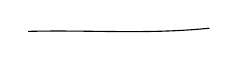
\begin{tikzpicture}\draw (0,0) .. controls (.8,.02) and (1.5,-.04) .. (2.3,.04);\end{tikzpicture}}
\mspage{362}
